\subsection{Descri\c c\~ao do problema} \label{subsec:descricao}

Para saber melhor o que está sendo trabalhado, a descrição do problema é um meio pelo qual as variáveis podem ser expostas e o que prever com o foco que está sendo abordado.
Se você não tiver um plano de previsão do que deve ser previsto, não faz muito sentido prever os dados usando modelos apenas para usá-los.

\begin{itemize}
	\item Bombas de sucção (B1, B2 e B3) – valor máximo da frequência 60 Hz
	
	\item[] Variáveis importantes: Fluxo, pressão e nível
	
	\item Nível do Reservatório (Câmara 1) LT01 $ (m^3) $ - \textbf{PREVER}
	
	\item Vazão de entrada (FT01) $ (m^3/h) $
	
	\item Vazão de gravidade (FT02) $ (m^3/h) $
	
	\item Vazão de recalque (FT03) $ (m^3/h) $
	
	\item Pressão de Sucção (PT01SU) (mca)
	
	\item Pressão de Recalque (PT02RBAL) (mca)
\end{itemize}

Na pesquisa, será usada a variável LT01, que é o nível do reservatório, nível esse de grande importância, conforme mostrado nas Figuras \ref{fig:dados-todos} e \ref{fig:2020-a-frente}. As Figuras retratam as anomalias ocorridas durante o período em que a capital paranaense sofreu com a falta de chuvas e o abastecimento dos reservatórios começou a reduzir o nível e enfrentar rodízios periódicos, conforme já comentado na subseção \ref{subsubsec:motivacao}. Com isso, pode-se entender melhor o que se espera daqui para frente.

\subsection{Procedimentos metodol{\'o}gicos} \label{subsec:metod}

Para prever e comparar cada modelo obtido na revisão sintemática para cada coisa, é definido um processo metodológico que será seguido, conforme mostrado abaixo na subseção \ref{subsubsec:etp} desta parte, pois o procedimento foi realizado desde o início, escolhendo o que prever, quais métodos usar para realizar a EDA devido à sequência que foi seguida.
   
    \subsubsection{Etapas da pesquisa}\label{subsubsec:etp}
    A pesquisa seguiu as seguintes etapas:
    \begin{figure}[H]
    	\centering
    	\caption{Mapa das Etapas}
    	\label{fig:etapas}
    	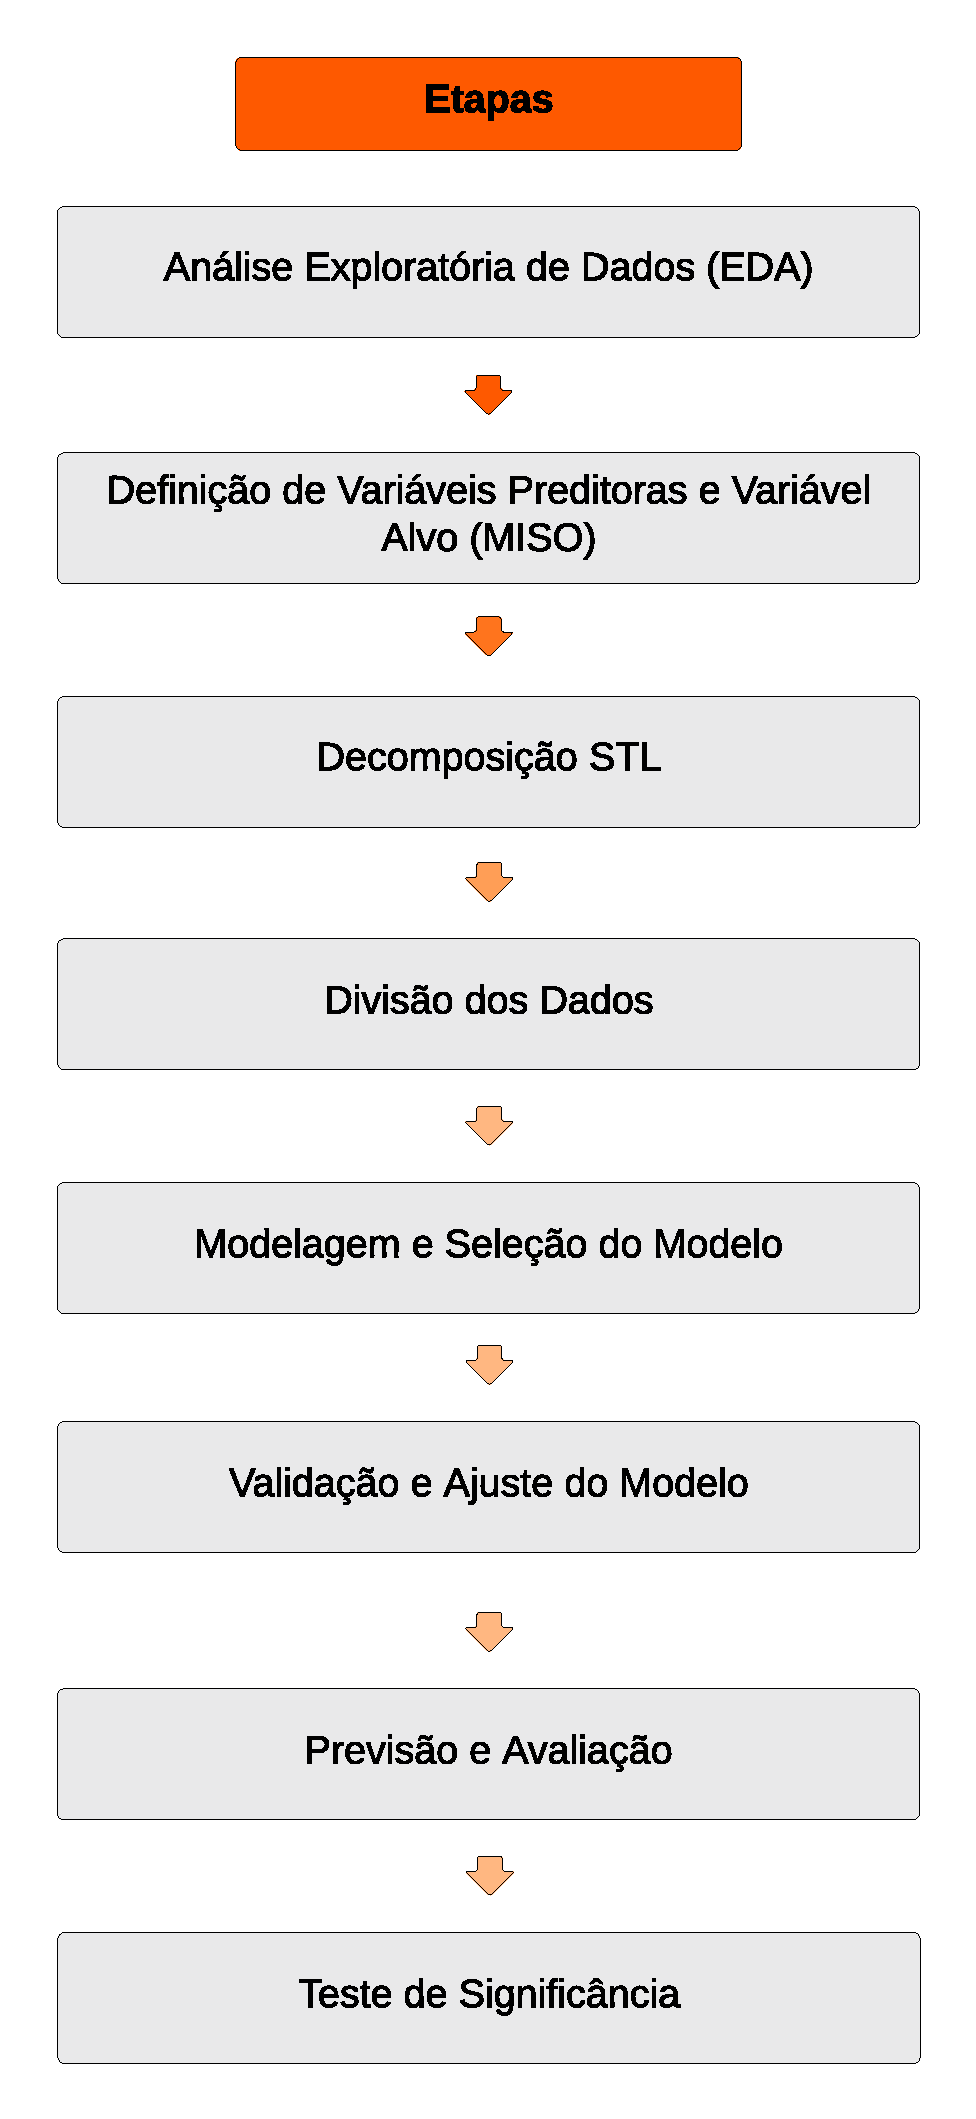
\includegraphics[width=0.9\linewidth]{Introducao/Figuras/Etapas}
    	
    	Fonte: Elaboração própria
    \end{figure}
    \begin{enumerate}[start=1, label = {\textbf{Etapa} \arabic* } ]
    	\item Análise exploratória dos dados – EDA ( do inglês \textit{Exploratory Data Analysis}). \label{etp:1}
    	
    	A exploração de dados na EDA é fundamental para entender melhor os dados que estão sendo trabalhados, como, por exemplo, excluir valores ausentes, saber como os dados estão separados em horas ou dias e, assim, tomar a melhor decisão a ser trabalhada com os dados, usar gráficos de linha na análise para observar a convergência dos dados e as anomalias que podem ocorrer.
    	
        	
    	\item O que vai ser usado como variáveis previsoras e qual será a variável a ser predita (MISO). \label{etp:2}
    	
    	Nessa etapa, tem o papel de relacionar as variáveis ao que será previsto, como os modelos de variáveis exógenas que são usados aqui nos modelos SARIMAX, ARX e ARIMAX do tipo ARIMA. Cada modelo tem a interação de mais variáveis do que o modelo ARIMA básico ou seus derivados AR, MA e SARIMA. O conhecimento de quais variáveis estão incluídas na modelagem do problema torna a modelagem mais abrangente quando o horizonte de previsão é estendido além dos dados.
    	
       	
    	\item Fazer a decomposição STL (do inglês \textit{Seasonal-Trend Decomposition}) Sazonalidade, Tendência e Resíduo. \label{etp:3}
    	
        O algoritmo STL executa suavização na série de tempo usando LOESS em dois loops; o loop interno itera entre a suavização sazonal e de tendência e o loop externo minimiza o efeito de valores atípicos. Durante o loop interno, o componente sazonal é calculado primeiro e removido para calcular o componente de tendência. O restante é calculado subtraindo os componentes sazonais e de tendência da série de tempo.
        
        Os três componentes da análise STL se relacionam com a série de tempo bruta da seguinte forma:
        
        \begin{eqnarray}
        	y_i &=& s_i + t_i + r_i
        \end{eqnarray}
    	
    	Onde:
    	
    	\begin{itemize}
    		\item $y_i = O$ valor da série de tempo no ponto $i$.
    		\item $s_i = O$ valor do componente sazonal no ponto $i$.
    		\item $t_i = O$ valor do componente de tendência no ponto $i$.
    		\item $ri = O$ valor do componente restante no ponto $i$.
    	\end{itemize}
    	\item \label{etp:4} Separação dos dados.
    	
    	Verifique a média e o desvio padrão de cada um desses conjuntos para obter a divisão mais adequada dos dados. Divida o conjunto de dados em treinamento, validação e teste. 70\% para treinamento e validação e 30\% para teste, a partir dessa divisão de 70\% em 80\% para treinamento e 20\% para validação.
    	
    	
    	\item Estratégia de previsão (recursiva e iterada-método direto). \label{etp:5}
    	
    	A estratégia recursiva envolve o uso de um modelo de uma etapa várias vezes, em que a previsão para a etapa de tempo anterior é usada como entrada para fazer uma previsão na próxima etapa de tempo.    	
    	No caso da previsão da demanda de água para os próximos dias, seria desenvolvido um modelo de previsão em uma etapa. Esse modelo seria usado para prever o dia 1 e, em seguida, essa previsão seria usada como uma observação para prever o dia 2.
    	    		 
    	Por Exemplo:
    	
    	\begin{eqnarray}
    	preditivo(t+1) &=& model_1(obs(t-1), obs(t-2), \ldots, obs(t-n))\\
    	preditivo(t+2) &=& model_2(obs(t-2), obs(t-3), \ldots, obs(t-n))   	
    	\end{eqnarray}
    	
    	\citeonline{machinemaster} como as previsões são usadas no lugar das observações, a estratégia recursiva permite que os erros de previsão se acumulem de tal forma que o desempenho possa se degradar rapidamente à medida que o horizonte de tempo de previsão aumenta.
    	
    	
    	\item Horizonte de previsão (1 passo ou n passos à frente). \label{etp:6}
    	
    	O tipo de horizonte foi escolhido de modo a mudar entre dias, prevendo um passo à frente, uma semana, duas semanas e um mês.
    	
    	
    	\item Modelos de previsão e métricas de desempenho. \label{etp:7}
    	
    	Os modelos discutidos aqui são os modelos clássicos de previsão, juntamente com os modelos de regressão gradiente. Os modelos são AR, ARX, ARMA, ARIMA, SARIMA, SARIMAX e ARIMAX, seguidos pelos modelos de regressão LR, XGBRegressor, RFR e LGBMRegressor. Esses modelos adotados foram escolhidos pela revisão sistemática realizada na dissertação.
    	
    	    	
    	As métricas usadas em toda a dissertação são as métricas RMSE, MAE e MAPE, encontradas na revisão e uma das mais usadas até hoje, na subseção \ref{subsec:metrica} é explicado em mais detalhes cada uma delas.
    	
    	
    	
    	%\item Ajustar os hiperparâmetros dos modelos de previsão Hiperparâmetro ajusta a priori (ex: número de neurônios da rede neural), e parâmetro (pesos da rede neural) ajusta durante o processo. \label{etp:8}
    	
    	
    	\item Aplicar os modelos de previsão e fazer comparativo baseado em testes de significância estatística (\textit{Friedman e Nemenyi}). \label{etp:9}
    	
    	
    	O teste de Friedman é o teste não paramétrico usado para comparar dados de amostras vinculadas, ou seja, quando o mesmo indivíduo é avaliado mais de uma vez. 
    	ou seja, quando o mesmo indivíduo é avaliado mais de uma vez. 
    	O teste de Friedman não usa os dados numéricos diretamente, mas sim as classificações ocupadas pelos dados após a classificação de cada grupo separadamente. 
    	separadamente. Após a classificação, a hipótese de igualdade da soma das classificações de cada grupo é testada. 

		O teste consiste em fazer comparações em pares com o intuito de verificar qual dos fatores que diferem entre si. No entanto, o teste de Nemenyi é muito conservador e pode não encontrar diferença significativa entre os pares testados.
    	
    \end{enumerate}






    